
\documentclass[12pt ]{iopart}
\usepackage{graphicx}
\usepackage{amsmath}
\usepackage[space]{grffile}
\usepackage{epstopdf}
\usepackage[autostyle,italian=guillemets]{csquotes}%bibliografia
%%\usepackage[bibstyle=authoryear,citestyle=authoryear-comp,backend=biber,uniquelist=false]{biblatex}%stile bibliografia
\usepackage[style=authoryear-icomp,maxbibnames=9,maxcitenames=1,uniquelist=false,
    backend=biber]{biblatex}

\usepackage{algorithm}
\usepackage[noend]{algpseudocode}

\addbibresource{b.bib}
%\newcommand{\gguide}{{\it Preparing graphics for IOP Publishing journals}}
%Uncomment next line if AMS fonts required
%\usepackage{iopams}  
\begin{document}

\title[DNN for EEG-fNIRS BCI]{Deep Learning for  hybrid EEG-fNIRS Brain Computer Interface: application to Motor Imagery Classification}

\author{Pierpaolo Croce\textsuperscript{1,2}, Filippo Zappasodi\textsuperscript{1,2}, Francesco di Pompeo\textsuperscript{1,2} Arcangelo Merla\textsuperscript{1,2} \& Antonio Maria Chiarelli\textsuperscript{1,2}}

\ead{pierpaolo.croce@unich.it}
\vspace{10pt}
\begin{indented}
\item[] \textsuperscript{1} Department of Neuroscience, Imaging and Clinical Sciences, "G.d’Annunzio" University, Chieti, Italy
\item[] \textsuperscript{2} Institute of Advanced Biomedical Technologies, "G.d’Annunzio" University, Chieti, Italy
\end{indented}

\begin{abstract}
	\\
	\textit{Objective.} Brain Computer Interface (BCI) refers to procedures that link central nervous system to a device.  BCI was historically performed using Electroencephalography. In the last years, the possibility of combining Electroencephalography with other neuroimaging technologies, such as functional Near Infrared Spectroscopy, was explored, obtaining increased performances. A crucial step of BCI is brain state classification from recorded signal features. Deep Artificial Neural Networks Classifiers recently reached unprecedented complex classification outcomes. These performances are achieved through increased computation power, efficient learning algorithms, valuable activation function, and restricted or back-fed neurons connections. By expecting significant overall BCI performances, we investigated the capabilities of combining multi modal Electroencephalography and functional Near Infrared Spectroscopy recordings with state-of the art Deep learning procedures.\\
	\textit{Approach.} We performed a guided Left and Right Hand Motor Imagery task on 6 subjects with a fixed classification response time of 1 second and overall experiment length of 10 minutes. Left vs. Right classification accuracy of the Deep Artificial Neural Network in the multimodal recording modality was estimated and it was compared to standalone EEG and different classifiers.\\
	\textit{Main Results.} At both a single subject and group level we obtained significant increase in performance when considering multimodal recordings and Deep Neural Network classifier with cumulative effects (ranging from a $3\%$ to a $24\%$ improvement in classification accuracy).\\
	\textit{Significance.} BCI performances can be drastically improved by employing multimodal recordings that provide electrical and hemodynamic brain activity information, in combination with advanced non-linear Deep Learning classification procedure.
\end{abstract}


\section{Introduction}

Brain Computer Interface (BCI) refers to a group of procedures that directly link  central nervous system to a computer or a device \parencite{wolpaw2000brain}. BCI can focus on mapping, assisting, augmenting, or repairing human cognitive and sensory-motor functions. 
Historically, BCI was performed using Electroencephalography (EEG) \parencite{lotte2007review}. EEG  provides information regarding brain electrical activity with very high temporal resolution (ms scale) \parencite{hallez2007review}. 

In the last years, BCI studies investigated the possibility of combining EEG with other neuroimaging technologies \parencite{pfurtscheller2010hybrid}. Among these, functional Near Infrared Spectroscopy (fNIRS) provided encouraging results \parencite{fazli2012enhanced}. 

EEG and fNIRS are both flexible, scalp located procedures that can be employed for monitoring multiple populations in ecological conditions \parencite{farroni2013infant, costantini2013studying, zappasodi2017prognostic, watanabe1999neonatal}. Whereas EEG captures the macroscopic temporal dynamics of brain electrical activity through passive voltages evaluation, fNIRS estimates brain hemodynamic oscillations  relying on spectroscopic measurements of oxy- and deoxy-hemoglobin (HbO and Hb, respectively) fluctuations in the cortex \parencite{villringer1997non, ferrari2012brief}. Orthogonally with respect to EEG, fNIRS, depending on the slow dynamics of the hemodynamic response, yields low temporal resolution but, because of the fast exponential decay of light sensitivity, it provides good spatial resolution (around 1 cm) \parencite{chiarelli2016combining, chiarelli2015comparison}. 

Because of different physiological information provided by and characteristic of EEG and fNIRS \parencite{croce2017exploiting}, higher BCI performances  of combined measurements with respect to standalone EEG were reported extensively \parencite{fazli2012enhanced, khan2014decoding, hong2015classification, chiarelliREVdaaggiungere} .

Two main processing steps are involved in BCI:  feature extraction and classification. 

EEG features are usually extracted based on the power of the signal frequency bands. Indeed, well-distinct behaviors of EEG signal have been identified based on signal frequencies (delta ($< 4 Hz$), theta ($4-7 Hz$), alpha ($8-15 Hz$), beta ($16-31 Hz$), and gamma ($> 31 Hz$) \parencite{nuwer1988quantitative}). For example, during the execution of a motor task (or during the imagination or observation of the movement), the beta activity is suppressed in related brain areas(Event Related Desynchronization, ERD) \parencite{pfurtscheller2001functional, pfurtscheller2006future}.  
fNIRS  features are generally  computed from  HbO and Hb variations in the brain which are dependent, among others, on the  Blood Oxygen Level Dependant (BOLD) effect \parencite{steinbrink2006illuminating, naseer2015fnirs}. 

The classification procedure aims at accurately classify the brain state  based on the extracted signal features  and it is a fundamental step of BCI processing.


Different  experiment and algorithms have been applied  to combined EEG-fNIRS BCI.  \textcite{Fazli_2012} proposed Linear Discriminant Analysis to classify ERD EEG and time average fNIRS concentration changes during executed movements as well as motor imagery.  In \textcite{ma2012hybrid} a Gaussian radial-basis kernel Support Vector Machine (SVM) was used to classify a motor imagery BCI based on EEG power spectral densities and fNIRS amplitude of the cerebral blood oxygen signal.   \textcite{lee2014hybrid} employed LDA on combined EEG and fNIRS features to classify three conditions: right and left motor imagery and idle status . They reached a classification accuracy of about $65\%$. In \textcite{buccino2016hybrid} the features to be submitted to a LDA were extracted combining two methods: Regularized Common Spatial Patterns (RCSP) for EEG and combination of average and slope indicators for fNIRS signals. In this case an accuracy between $72-79\%$ was reached in a movement recognition task. In  \textcite{khan2014decoding, khan2017hybrid} LDA was used to classify control commands based on EEG peak amplitudes of selected motor area channels and mean values of HbO and Hb for fNIRS with accuracy ranging between $80-95\%$.
For all of the above mentioned studies, the authors recognized and increase BCI performance of combined measurements with respect to standalone fNIRS and EEG.

Recently, Deep Learning Classifiers are increasing their popularity. In the simplest fashion, Deep Learning  refers to Artificial Neural Networks (NN) \parencite{lecun2015deep, schmidhuber2015deep} that are composed of many layers. Deep NNs (DNN) use a cascade of  layers of nonlinear processing units (neurons). Each successive layer uses the output from the previous layer as input and all, or part, of the neurons from consecutive layers are connected. DNN can perform very complex, non-linear, transformations-classifications, greatly increasing shallow NN  \parencite{bianchini2014complexity}  and other classifiers performances (LDA, SVM, etc.). In fact, they can reach unprecedented classification outcomes when applied to signals (e.g. speech and language processing ) and or images \parencite{simonyan2014very, hinton2012deep, collobert2008unified, krizhevsky2012imagenet}. Because of their performances, these algorithms are also receiving  attention within the biomedical field \parencite{ronneberger2015u, hudson2000neural, ciresan2012deep}. 
Multiple technological development allowed for Deep learning evolution. 
Among them, the increased computation power clearly played an important role.
However, the major improvements are algorithms related and they can be divided in three  categories:

\begin{itemize}
	\item[-] Implementation of Efficient learning algorithms that avoid local minima in the objective function and poor generalization (over-fitting) \parencite{kingma2014adam} ; because of the presence of many free parameters (sometimes millions or more), and the possibility to represent very complex functions, DNN were usually affected by local minima in the objective function and over-fitting  during training. 
	\item[-] Development of new Neuron's activation functions (such as Rectified Linear Unit Function, ReLU function \parencite{dahl2013improving, maas2013rectifier}) that dampen  the vanishing gradient problem \parencite{pascanu2013difficulty}; in fact traditional activation functions such as the hyperbolic tangent or the sigmoid functions had wide ranges of the independent variables with small gradients;  this aspect, combined with the back propagation algorithm \parencite{hecht1988theory}, exponentially dampened weight update rate going from the last to the first layers, heavily slowing the overall learning rate of the network.
	\item[-] Implementation of  Neural Networks were Neurons are connected to portions of signals and or images that are close in time and/or space (Convolutional Neural Networks, CNNs \parencite{krizhevsky2012imagenet, kalchbrenner2014convolutional}), encoding temporal and/or spatial information; standard, full connected DNN  did not encode any spatio-temporal information.
	\item[-] Development of  Neural Networks were outputs are fed back into the network in a sequential manner that allow information storage (Recurrent Neural Networks, RNNs \parencite{mikolov2010recurrent, hochreiter1997long}). Standard, full connected DNN  did not provide memory capabilities and sequential information control.
\end{itemize}

DNN have been successfully applied to  both EEG and fNIRS BCI classification problem. In \textcite{jirayucharoensak2014eeg} a Deep Learning Network was used to classify three levels of valence and arousal based on EEG power spectral densities  features. They reached an accuracy of about $50\%$. 
\textcite{hajinoroozi2015feature} employed Deep Belief Network to EEG signals for the classification of driver's cognitive states. 
In \textcite{an2014deep} left vs. right motor imagery classification  was performed by employing few EEG recording channels via DNN with an average accuracy of about $80\%$ . 
 \textcite{bashivan2015learning} trained a CNN using EEG power in three different frequency bands of interest. They reported a best-performance accuracy of about $92\%$.

Regarding fNIRS, only  few  studies were performed employing Deep Learning.  \textcite{hennrich2015investigating} investigated DNN classification performances of three mental task reporting accuracy values similar  to other classification algorithms (such as LDA and SVM).  \textcite{abibullaev2011neural} classified four mental task through DNN with an accuracy of $94\%$. Finally, \textcite{nguyen2013temporal} classified Left vs. Right motor imagery fNIRS activity with average accuracy of $85\%$. To the best of our knowledge, no studies implementing deep learning algorithm for BCI classifications  in a combined EEG-fNIRS framework were performed.

In this paper, by expecting significant overall BCI performances,  we investigated the capabilities of combining multi modal EEG-fNIRS brain recordings  with state-of the art Deep learning Classification procedures. As a first investigation step, we performed a guided Left and Right Hand Motor Imagery task \parencite{pfurtscheller1997motor} and, by employing a common temporal frame of 1 second between technologies \parencite{govindan2016novel}, Left vs Right classification accuracy of a DNN in in the multimodal recording modality was estimated and compared to other classification algorithms and to standalone EEG. 

\begin{figure}
	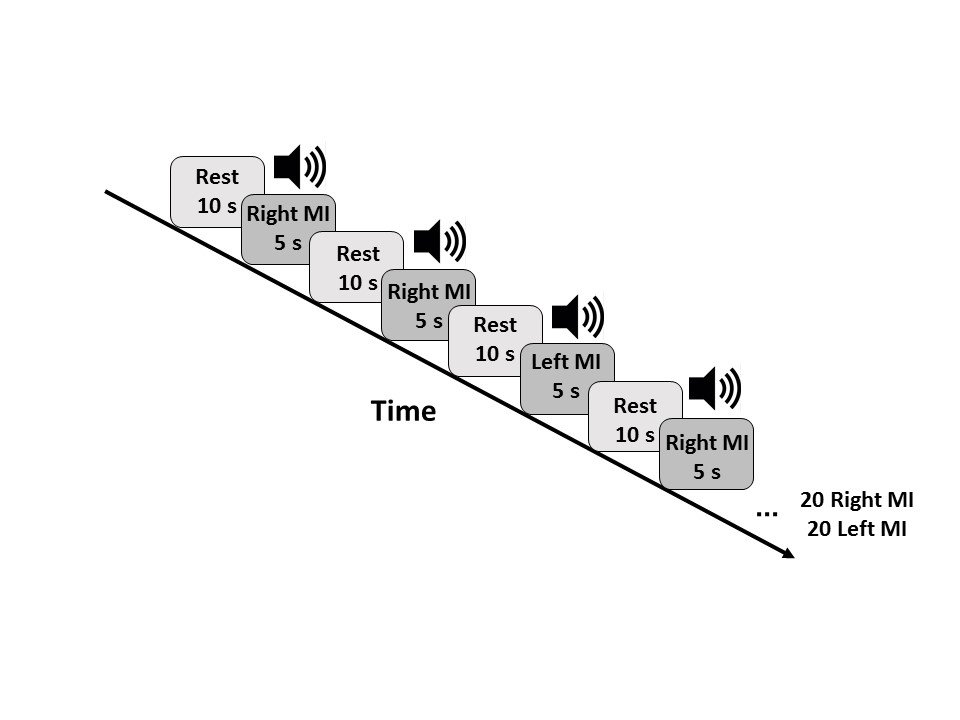
\includegraphics[width=\linewidth]{Slide1.JPG}
	\caption{ Motor imagery task sequence. The 
		squeezing imagery consisted of 5 seconds of task and 10 seconds of rest. Right or Left imagery instruction was presented in a pseudo-random order.  During the 5 seconds of task, the subjects were instructed to perform the squeezing imagery with a repetition frequency of $\sim1Hz$. The task provided a total number of 20 Left-hand and 20 Right-Hand 5 seconds trials in an experiment time of 10 minutes. }
	\label{fig:fig1}
\end{figure}

\section{Methods}
\subsection{Experimental Paradigm}
Six healthy subjects (males, average age of $34$ years $\pm$ $5$ years) were recruited for the study. All subjects were right handed, reported no history of neurological or psychiatric disease and did not receive psychoactive medications. 
Subjects set on a chair with the arms comfortably resting on a desk and were asked to perform right or left hand squeezing imagery guided by an acoustic stimulus. The motor imagery task sequence is depicted in figure \ref{fig:fig1}. The 
squeezing imagery consisted of 5 seconds of task and 10 seconds of rest. Right or Left imagery instruction was presented in a pseudo-random order.  During the 5 seconds of task, the subjects were instructed to perform the squeezing imagery with a repetition frequency of $\sim1Hz$. The task provided a total number of 20 Left-hand and 20 Right-Hand 5 seconds trials in an experiment time of 10 minutes. 

\begin{figure}
	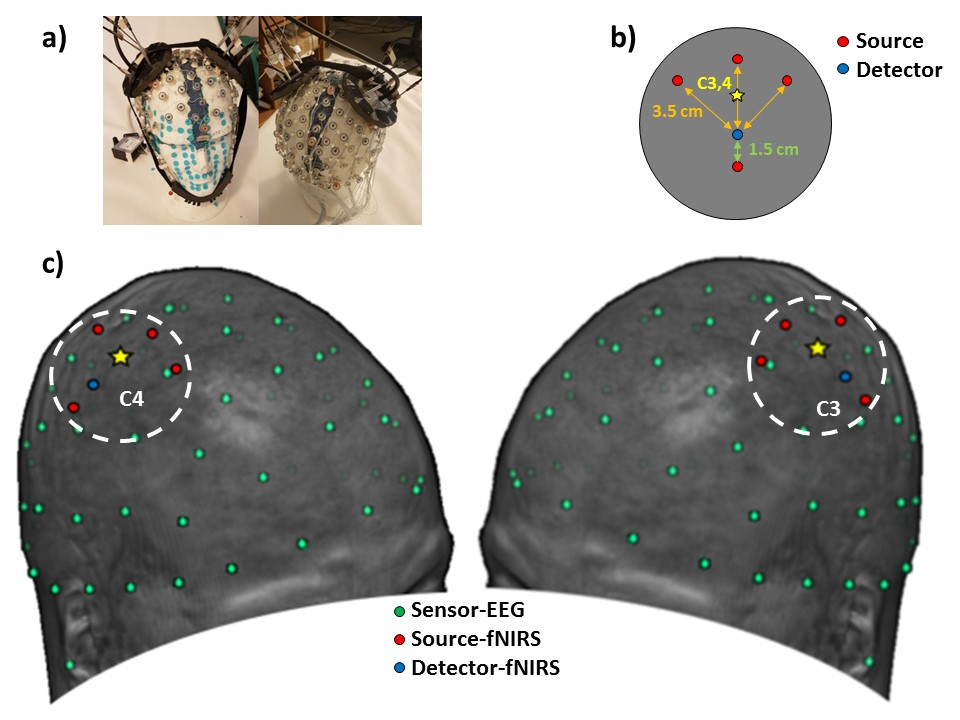
\includegraphics[width=\linewidth]{Slide2.JPG}
	\caption{a) Pictures of the full head EEG cap and optical probes located on a dummy head. The EEG was a Electrical Geodesic Net 300 system. The fNIRS spectrometer was an Imagent from ISS with 32 laser diodes and 4 PMTs. Light was sent to the scalp using multimodal optical fibers (0.4 mm core) and from the scalp back to the PMTs using fiber bundles (3 mm diameter).  The fibers were held in place using soft, but rigid, custom-built optical patches located on top of the EEG. b) Optical layout employed for each hemisphere. The optical layout consisted of 3 fNIRS channels over C3 and C4 with an interoptode distance (3.5 cm) that allowed sensitivity to brain activity. One short distance channel (1.5 cm),  not sensitive to brain activity (its sensitivity pattern does not reach the brain cortex), provided information regarding scalp-related hemodynamic oscillations. c) EEG electrodes and fNIRS optodes employed in the study overlayed onto a rendered structural Magnetic Resonance Image of a representative subject. }
	\label{fig:fig2}
\end{figure}


\subsection{ElectroEncephalography Recordings}
Brain electric activity was recorded with a full-head 128 channels EEG system (Electrical Geodesic Inc, EEG System Net 300, figure \ref{fig:fig1}a,c.).
Skin/electrode impedance was measured before recordings and kept below $50 k\Omega$. EEG data were sampled at 250 Hz and processed in a real time fashion.  Raw data were stored over 1 second window and filtered between 13 Hz and 30 Hz (2nd order Digital Butterworth filter). The beta-band filtered signal was squared and averaged over the second ($\beta_{Pow}$).
 The Event-Related Synchronizations (ERSs) or Event-Related Desynchronizations (ERDs) (Pfurtscheller and Lopes da Silva, 1999; Neuper and Pfurtscheller, 2001) were obtained as relative changes in power during the motor imagery execution with respect to rest:

\begin{equation}
\label{eqn:erders}
ERD/ERS=\frac{\beta_{PowMI}-\beta_{PowBas}}{\beta_{PowBas}}
\end{equation} 

where $\beta_{PowMI}$ is the average power over 1 second window during the task and $\beta_{PowBas}$ is the average power in a 1 second window prior to the task onset.
ERD/ERS values for each second during the task were fed to the learning algorithms for classification. Only 123 of the 128 EEG electrodes were employed in the learning process (5 auxiliary signal electrodes were removed).

\subsection{functional Near Infared Spectroscopy Recordings}
Brain hemodynamic activity was recorded over the sensorimotor regions (C3 and C4, 10-20 System) employing a commercial NIR spectrometer from ISS (Imagent™, Champaign, Illinois).
The apparatus is a Frequency Domain system equipped with 32 laser diodes ($\sim$1 mW  power, 16 emitting light at 690 nm and 16 at 830 nm) and 4 photo-multiplier tubes (PMTs). 
8 light sources (4 injection point, 2 wavelengths) and 1 detectors were employed for each hemisphere. Time-multiplexing was employed for source coding with a total system sampling frequency of 10 Hz.  Light was sent to the scalp using multimodal optical fibers (0.4 mm core) and from the scalp back to the PMTs using fiber bundles (3 mm diameter).  The fibers were held in place using soft, but rigid, custom-built optical patches located on top of the EEG, figure \ref{fig:fig1}a, with an optical layout reported in figure \ref{fig:fig1}b, c. The optical layout consisted of 3 fNIRS channels over C3 and C4 with an interoptode distance (3.5 cm) that allowed sensitivity to brain activity. One short distance channel (1.5 cm),  not sensitive to brain activity (its sensitivity pattern does not reach the brain cortex), provided information regarding scalp-related hemodynamic oscillations \parencite{gagnon2014further}.  
The raw Continuous Wave intensity ($I$)  was averaged  at a 1 sec pace .
The optical densities (ODs)over time were computed as:

\begin{equation}
\label{eqn:erders}
OD=-\ln\frac{I(t)}{I(t_{0})}
\end{equation} 

where $I(t)$ is the signal intensity at second t and $I(t_{0})$ is the average signal intensity in the first second of recording.
Variations in the concentration of oxy-hemoglobin and deoxy-hemoglobin were derived for each channel  based on the Modified Lambert Beer Law \parencite{sassaroli2004comment}:

\begin{equation}
\begin{bmatrix}
O_2Hb\\
HHb
\end{bmatrix}
=
\frac{1}{\rho}\begin{bmatrix}
\epsilon_{O_2Hb}(\lambda_1)\cdot DPF(\lambda_1)&\epsilon_{HHb}(\lambda_1)\cdot DPF(\lambda_1)\\
\epsilon_{O_2Hb}(\lambda_2)\cdot DPF(\lambda_2)&\epsilon_{HHb}(\lambda_2)\cdot DPF(\lambda_2)
\end{bmatrix}^{-1}\times
\begin{bmatrix}
OD(\lambda_1)&\\
OD(\lambda_2)
\end{bmatrix}
.
\end{equation}

where $O_{2}Hb$ and $HHb$ represent the changes in oxy-hemoglobin and deoxy-hemoglobin concentrations , $\rho$ is the interoptode distance, $\epsilon$  and DPF are, respectively, the extinction coefficients for the two chromophores and the Differential Pathlength Factors at the wavelengths of interest ($\lambda _{1}$ and $\lambda _{2}$). The extinction coefficients of the two forms of hemoglobin at the different wavelengths  were extracted from \parencite{zijlstra1991absorption} ( $\epsilon_{O_{2}Hb}(690nm)$ = 0.0096 $mm^{-1}$, $\epsilon_{O_{2}Hb}(830nm)$ = 0.021 $mm^{-1}$, $\epsilon_{HHb}(690nm)$ = 0.05 $mm^{-1}$, $\epsilon_{HHb}(830nm)$ = 0.017 $mm^{-1}$).  The DPFs were derived fron Scholkmann and Wolf  ( $DPF(690nm)$ = 6.5, $DPF(830nm)$ = 5.5) \parencite{scholkmann2013general}.
Oxy-hemoglobin $\Delta O_{2}Hb$ and deoxy-hemoglobin $\Delta HHb$ changes during the motor imagery were obtained  with respect to rest (8 channels and 2 Hemoglobin forms for a total of 16 features per second):

 \begin{equation}
\begin{bmatrix}
\Delta O_2Hb\\
\Delta HHb
\end{bmatrix}
=
\begin{bmatrix}
O_2Hb_{MI}-O_2Hb_{Bas}\\
HHb_{MI}-HHb_{Bas}
\end{bmatrix}
.
\end{equation}

where $O_{2}Hb_{MI}$ and $HHb_{MI}$ are the average hemoglobin concentrations over 1 second window during the task and $O_{2}Hb_{Bas}$ and $HHb_{Bas}$ are the average hemoglobin concentrations in a 1 second window prior to the task onset.
Hemoglobin change  in both short and long distance channels for each second during the task were fed to the learning algorithms for classification. 

\begin{figure}
	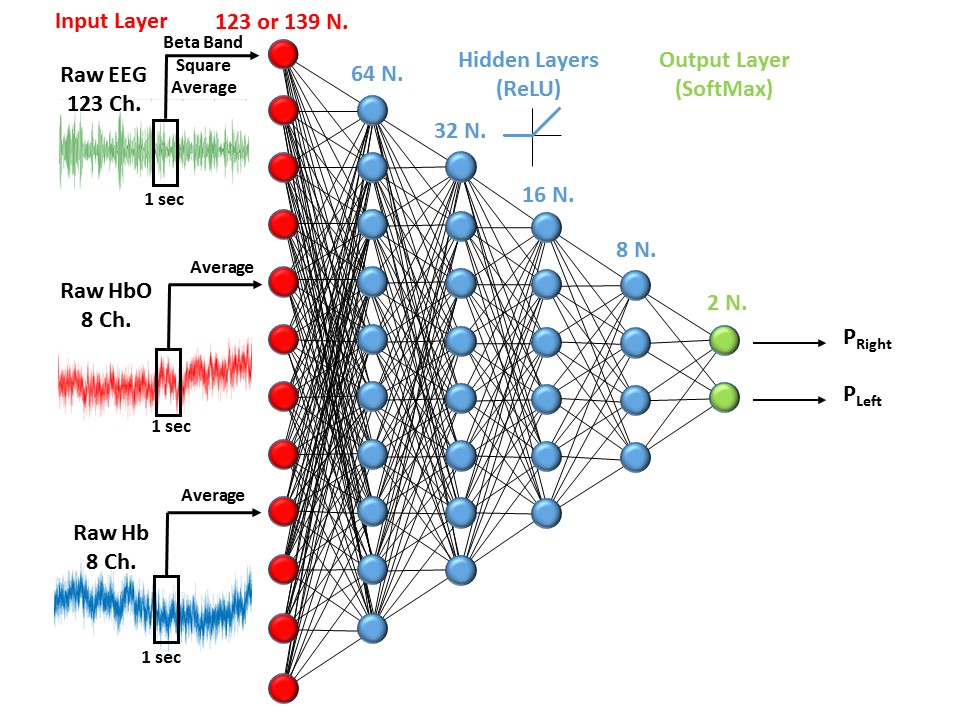
\includegraphics[width=\linewidth]{Slide3.JPG}
	\caption{DNN Network employed for motor imagery classification. The network was a full connected feed-forward  DNN . Input neurons were 123 (when standalone EEG classification was performed), or 139 (when both EEG and fNIRS were employed). 
	The feature of the input neurons were 1 second average ERD/ERS, $\Delta O_{2}Hb$ and $\Delta HHb$, expressed in microMolar ($\mu M$) change. 
	 As a non-linear processing function of the neurons' hidden layers the Rectified Linear Unit (ReLU) function was employed. 
	 The number of hidden layers (4) and neurons were selected to approximately decrease the number of processing unit ( thus compressing information) by a factor of 2 between successive layers. The output layer was composed of two neurons performing a softmax transformation. The softmax function outputs for the two neurons  the predicted probability of being in the right ($P_{Right}$) or left ($P_{Left}$) imagery state. }
	\label{fig:fig3}
\end{figure}

\subsection{Deep Neural Networks and Classification}
Deep Neural Networks (DNNs) allow computational models that are composed of multiple  processing layers of non-linear units, called neurons, able to learn representations of data with multiple levels of abstraction.
Deep Neural Networks find complex structure in  data-sets by using the backpropagation algorithm \parencite{hecht1988theory} that guides changes in Networks' parameters that are sequentially updated in each layer from the representation in the previous layer.
Whereas Network parameters are learned from the data, the DNN structure have to be heuristically selected a priori or determined through computationally demanding hyper parameters optimization algorithms %\parencite{mackay1996hyperparameters} \parencite{snoek2012practical} \parencite{bengio2000gradient}.
\parencite{mackay1996hyperparameters,snoek2012practical,bengio2000gradient}
Since we performed a first investigatory comparison between DNN performance and other classifier performances, we decided to fix the DNN structure (also called the DNN hyperparameters), without investigating multiple DNN architectures.
The Network employed was a full connected feed-forward DNN and its structure is reported in figure \ref{fig:fig3}
Our data set consisted of 123 (when standalone EEG classification was performed), or 139 (when both EEG and fNIRS were employed) input neurons. 
The feature of the input neurons were 1 second average ERD/ERS, $\Delta O_{2}Hb$ and $\Delta HHb$, expressed in microMolar ($\mu M$) change. Notice that the average value of the features were of the order of 1 and all features' values were within one order of magnitude. This is an important aspect to account when training DNNs.
Each neuron of the hidden layers performs a non-linear transformation of a linear combination of all the output from the previous layer. As a non-linear processing function we decided to employ the Rectified Linear Unit (ReLU) function, which was proven to dampen the vanishing gradient problem providing better performance than other non-linear functions (such as the hyperbolic tangent or the sigmoid functions) \parencite{dahl2013improving}. Hidden neurons response  when ReLU is employed can be written as:

\begin{equation}
y=
\begin{cases}
0,& \text{if } wx+b \leq 0\\
wx+b,&\text{if } wx+b > 0
\end{cases}
\end{equation}

where $x$ is the input vector, $w$ and $b$ are the weight vector and bias , respectively, and $y$ is the output vector.
Since the classifier had to discriminate between two states, namely Left or Right Motor Imagery state, the output layer was composed of two neurons performing a softmax transformation:

\begin{equation}
\begin{bmatrix}
P_{Right}\\
P_{Left}
\end{bmatrix}
=
\begin{bmatrix}
\frac{e^{w_1x}}{\sum\limits_{k=1}^2 e^{w_kx}}\\
\frac{e^{w_2x}}{\sum\limits_{k=1}^2 e^{w_kx}}
\end{bmatrix}
.
\end{equation}

The softmax function outputs for the two neurons  the predicted probability of being in the right ($P_{Right}$) or left ($P_{Left}$) imagery state. 
$x$ is the input vector of the softmax layer and $W_{1}$ and $W_2(2)$ are the weight vectors of the neurons.
The number of hidden layers (4) and neurons (refer to figure \ref{fig:fig3}) were selected to approximately decrease the number of processing unit ( thus compressing information) by a factor of 2 between successive layers. 
The weights were initialized in a pseudo-random approach employing a truncated normal distribution (0 mean, 0.1 SD, 2 SD truncation), whereas the biases were initialized to 0. Random initialization of weights was proven to be another factor that avoids local minima during training \parencite{sutskever2013importance}.

The DNN was trained in a supervised learning approach \parencite{hastie2009overview}.
In the supervised learning, DNN parameters, i.e. weights $w$s and biases $b$s, are adjusted relying on an objective function minimization procedure. The objective function measures the error (or distance) between the output scores and the desired scores . We employed the cross-entropy error as objective function.
Cross-entropy (CE) is defined as:

\begin{equation}
CE=
-\sum\limits_i y'_{i}\ln y_{i}
\end{equation}

where $y$ is the output vector of the DNN ([$P_{Right}$  $P_{Left}$] in the study) $y'$ is the known state ([1 0] for Right Hand Imagery or [0 1] for Left Hand Imagery)
 Cross-entropy metric takes into account the closeness of a prediction and is a more granular way to compute error than Classification Error or Mean Squared Error \parencite{murphy2012machine}.
 
 The choice of optimization algorithm for deep learning model is extremely important.
 In general,  learning algorithms optimize network's weights and biases by exploring the space of such parameters relying on local the slope (gradient) of the objective function.  
 As optimization algorithm we employed the state-of the art Adam Optimizer \parencite{kingma2014adam}.
Adam Optimizer is an algorithm that is different from classical stochastic gradient descent since the methods computes individual adaptive learning rates for different parameters from estimates of first and second moments of the gradients.
Adam Optimizer parameters were set to: learning rate=$10^{-4}$, first moment exponential decay rate=$9\cdot 10^{-1}$,  second moment exponential decay rate=$9.99\cdot 10^{-1}$, constant=$10^{-8}$ \parencite{kingma2014adam}.
The optimization procedure was iterated for 1000 epochs.
In order to address the DNN performance, we decided to perform a 10-fold cross validation procedure \parencite{kohavi1995study} employing all the 200 seconds of Right or Left motor imagery for each subject. 
The training and testing set for each validation were selected from different imagery trials.
The cross-validation procedure was performed 1000 times. 
This analysis provided an estimate of the performance achieved by the DNN after a training of $\sim$9 minutes employing the chosen task design. 
The accuracy of the DNN was evaluated by counting the number of correct DNN predictions after an argmax evaluation of probabilities of the DNN output vector.
The described DNN architecture, training and validation were implemented in Python  through the open-source software library Tensorflow \parencite{abadi2016tensorflow}.
DNN performances were compared to LDA and linear SVM.
LDA is a classical closed-solution linear classificator that rely on classes means and covarancies \parencite{balakrishnama1998linear}.
SVM is a supervised learning algorithm that can be employed for binary linear classification. SVM model is a representation of  points in the feature space, mapped so that the points of different classes are divided by a gap that is as wide as possible \parencite{cortes1995support}.
LDA and SVM performances were estimated employing  a 10-fold cross validation procedure. In accordance with the DNN analysis,  the cross-validation procedure was performed 1000 times. 
LDA ans SVM analysis were performed in Matlab.

\subsection{Statistical Analysis}

The statistical analysis was threefold:
\begin{itemize}
\item It compared multimodal EEG-fNIRS with standalone EEG  BCI performances (it estimated the Recording Effect);
\item It compared DNN with other classification  algorithms (LDA and SVM, it estimated the Classificator Effect).
\item It investigated possible interactions or cumulative effects between the Recording and the Classificator Effects.
Results from the 6 subjects (classification accuracy) were computed for all possible combination of recordings and classificators. 
Since standalone EEG recordings coupled with LDA classificator can be considered the simplest BCI configuration, the analysis that investigated main effects and interactions of recording modality and classificator were performed on differential accuracies with respect to EEG-LDA.
This differential analysis was conducted to dampen the problem of the intrinsic variability of  the classification outcome among subjects, highlighting changes in accuracy caused by  Recording and the Classificator modalities.
A two-way anova was performed to investigate possible main effects and interactions of Recording  (factor one, EEG vs. EEG-fNIRS with respect to EEG-LDA), and  Classificator (factor two, SVM vs. DNN with respect to EEG-LDA) at a subjects' group level.
Moreover, post-hoc analysis were conducted to provide average differences and their statistical significance among different conditions.
Statistical analysis was performed in Matlab.
\end{itemize} 

\begin{figure}
	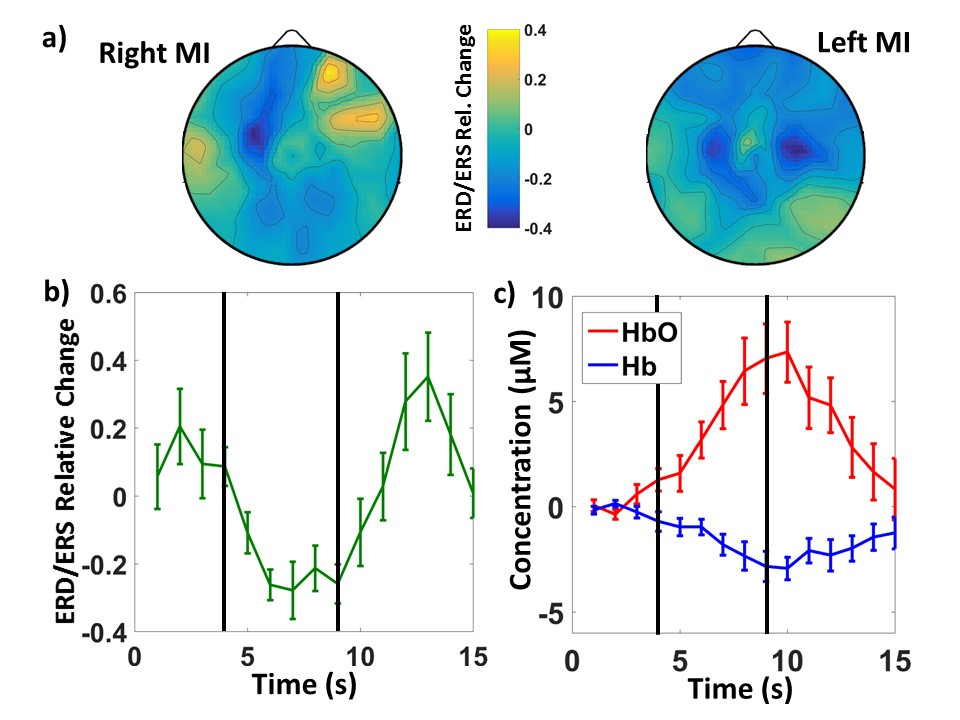
\includegraphics[width=\linewidth]{Slide4.JPG}
	\caption{a) Examples of average EEG Right and Left Motor Imagery responses for a representative subject across all the 20 trials.
	The motor cortex controlateral ERD activation (lower $\beta$ power with respect to baseline) is appreciable. b) Average timecourse and related standard errors of the ERD/ERS relative change from 5 seconds prior to 5 seconds post right motor imagery task for the same subject in a highly activated electrode located over the left sensorimotor cortex. c)  Average timecourses and related standard errors of $O_{2}Hb$ and $HHb$ change from 5 seconds prior to 5 seconds post right motor imagery task for the same subject in an activated left located channel for the same subject.}
	\label{fig:fig4}
\end{figure}

\begin{figure}
	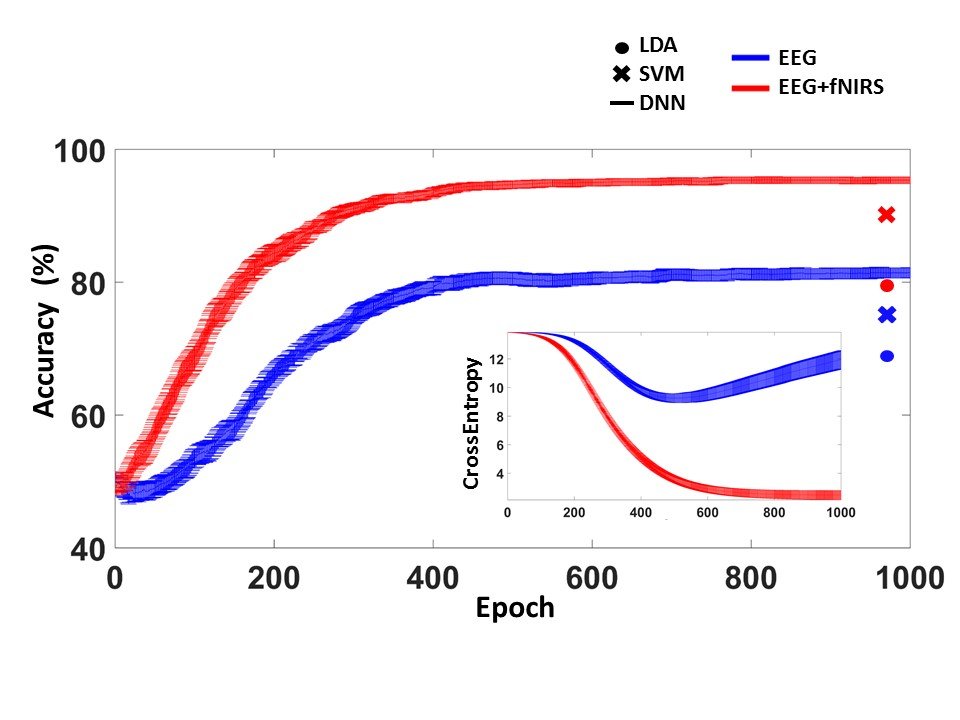
\includegraphics[width=\linewidth]{Slide5.JPG}
	\caption{Average accuracy and related standard errors
		of the DNN employed as a function of training epoch when standalone EEG or combined EEG-fNIRS recordings were analyzed. The average accuracy and variability were computed among cross-validations. 
		The figure also reports related cross-entropies estimates, along with 
		cross-validated LDA and SVM average accuracies.}
	\label{fig:fig5}
\end{figure}

\begin{figure}
	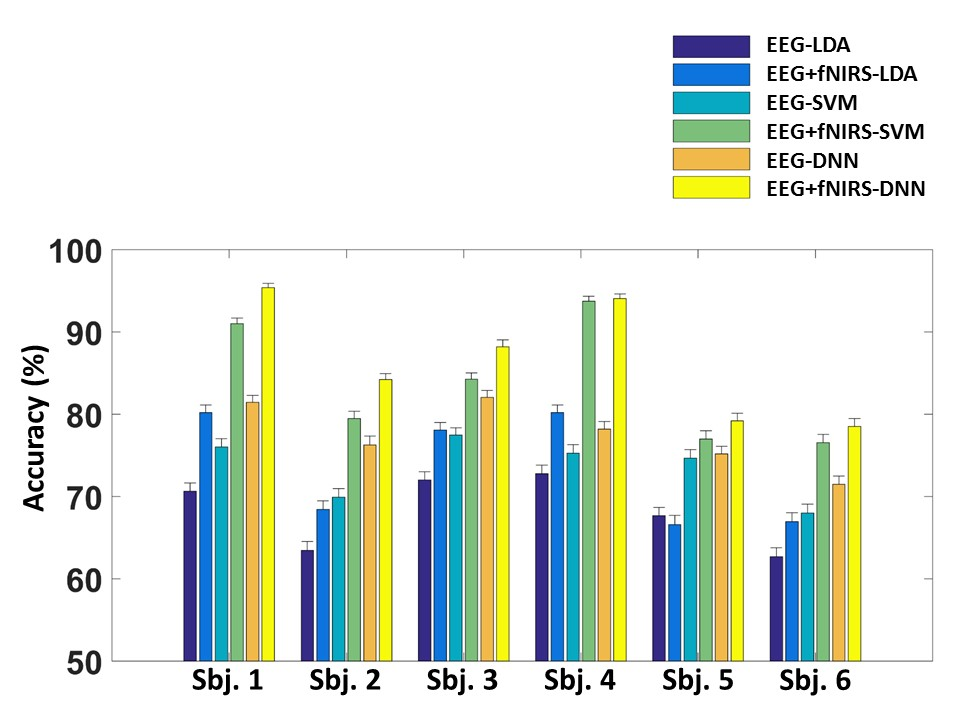
\includegraphics[width=\linewidth]{Slide6.JPG}
	\caption{Average and related standard errors of cross-validated accuracies of all combination of recording procedure and classificator technology for each of the six subjects.}
	\label{fig:fig6}
\end{figure}

\section{Results}
Figure \ref{fig:fig4}a shows examples of average Right and Left Motor Imagery responses for a representative subject across all the 20 trials.
A typical controlateral ERD activation (lower $\beta$ power with respect to baseline) on the motor cortices is appreciable.
Figure \ref{fig:fig4}b shows the average timecourse and related standard errors of the ERD/ERS relative change from 5 seconds prior to 5 seconds post to the right motor imagery task for the same subject in a highly activated electrode located over the left sensorimotor cortex .Figure \ref{fig:fig4}c shows the average timecourses and related standard errors of oxy- and deoxy-hemoglobin changes considering the same time frame in an activated left-located channel during Right hand MI. A typical Blood-Oxygen-Level Dependent (BOLD) effect can be identified in response to the motor imagery. 
Figure \ref{fig:fig5} show average accuracy performances and related standard errors
of the DNN employed as a function of training epoch when standalone EEG or combined EEG-fNIRS recordings were analyzed. The average accuracy and variability were computed among cross-validations. 
Figure \ref{fig:fig5} also reports related cross-entropies estimates.
Moreover, LDA and SVM average cross-validated performances are reported on top-right corner of the figure.
For the reported subject, which was the one providing the overall highest classification performance, a clear increase in accuracy can be appreciated when fNIRS is employed with EEG ($95.40\%$ with respect to standalone EEG, $81.50\%$), independently of the classificator, and a clear different performance of classification accuracy as a function of classificator (LDA,SVM, DNN in increasing classification accuracy order), independently of the recording procedure with apparent cumulative effects.
Figure \ref{fig:fig6} reports the average and related standard errors, cross-validated accuracies of all combination of recording procedure and classificator technology for each of the six subjects. A similar pattern as the one reported for the representative subject in figure \ref{fig:fig5} is present for all of the subjects examined.
However, a clear variance in the average classification performance among subjects is appreciable with a best intra-subject performance ranging from $78.50\%$ to $95.40\%$. 
Thus, in order to highlight specific effects of recordings and classificator the two way anova described in the Statistical Analysis section was performed on accuracies increases with respect to EEG-LDA. Before the anova, a Shapiro-Wilk normality test proved the gaussian-like distributions of the accuracy changes within each conditions (all p's$>$0.05).
The two-way anova highlighted a strong effect of Recording (F(1,20)=42.22, p$<$0.05) and a significant effect of Classificator (F(1,20)=5.27, p$<$0.05). No interaction between Recording and Classificator was found (F(1,20)=0.11, p$>$0.05). The anova results suggest a main effects of both Classificator procedure and recording on the accuracy of the BCI with a possible cumulative effect without interaction.
Post-hoc analysis tested pairwise differences  of conditions and it provided statistical significance for practically  all possible combinations (p's$<$0.05).
We obtained an average increase of EEG-SVM with respect to EEG-LDA of $5.35\%$ (SD=$1.56\%$), an increase of EEG+fNIRS-SVM of $15.47\%$ (SD=$4.58\%$), an increase of EEG-DNN of $9.24\%$ (SD=$2.59\%$) and an increase of EEG+fNIRS-DNN of $18.39\%$ (SD=$4.75\%$). Notably the increase in accuracy from EEG to EEG+fNIRS, without considering classificator, was of $9.63\%$, whereas the increase in accuracy from SVM to DNN, without considering recordings, was of  $3.41\%$. This results, combined with an overall increase of EEG+fNIRS-DNN vs EEG-SVM of  $13.04\%$ highlighted the cumulative effect of multimodal recording and DNN classification procedure.

\section{Discussion}
Short re-caption of main DNN concepts and EEG-fNIRS for MI.
Discussion of obtained results:
increased performance with fNIRS and with DNN classification without interaction (cumulative effect).
Non linear space separation complex, 
In addition to performing linear classification, SVMs can efficiently perform  non-linear classification by mapping their inputs into high-dimensional feature spaces.
We tried radial basis
Limitations: fixed hyperparameters
(overall length of experiment, frequency band, response time (1sec), DNN structure). 
Report spatial CNN results were poorer (low spatial information content of EEG), may work better with full-head fNIRS. Time CNN for feature extration worked not well
Future direction RNN for self paced


\section{Conclusion}

\section{Acknowledgements}
This study was partially funded by grant: H2020, ECSEL-04-2015-Smart Health, Advancing Smart Optical Imaging and Sensing for Health (ASTONISH).
 

\newpage
\printbibliography
\cleardoublepage
\addcontentsline{toc}{section}{\refname}
\end{document}
